\subsection{23.11.18}
\subsubsection{Задача о медицинском обследовании}
Пусть существует некая болезнь "СПИД ноги", которой подвержены $10\%$ населения. \\
Есть тест на выявление этой болезни, который: \\
\begin{itemize}
\item Имеет $10\%$ вероятность ложного отрицания (вероятность отрицательного (N) результата теста, если человек болен (S)).\\
\item Имеет $30\%$ вероятность ложного подтверждения (вероятность положительного (P) результата теста, если человек здоров (H)).\\
\end{itemize}
Построим дерево вариантов:\\
\begin{figure}
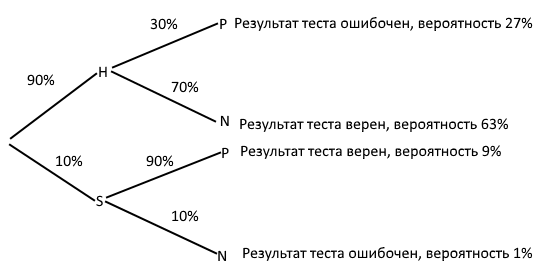
\includegraphics[width=\linewidth]{Medicare.png}
\caption{Дерево вариантов}
\label{fig:Medicare}
\end{figure}
Посчитаем несколько вероятностей:\\
\begin{itemize}
\item $Pr\{$Тест положительный$\} = Pr(\{HP, SP\}) = 9\% + 27\% = 36\%$. то есть, несмотря на то, что болеет всего $10\%$ населения, тест даст положительный результат более чем в $\frac{1}{3}$ случаев.\\
\item $Pr\{$Человек болен, если тест положительный$\} = Pr(\{SP, SN\}|\{HP, SP\}) = \frac{Pr(\{SP\})}{Pr(\{HP, SP\})} = \frac{9\%}{36\%} = 25\%$\\
\item $Pr\{$Тест работает верно$\} = Pr(\{HN, SP\}) = 63\% + 9\% = 72\%$
\end{itemize}
Кажется, что тест не очень эффективен. Но так ли это?\\
Рассмотрим инновационный тест (спонсированный военкоматом), который всегда выдает отрицательный результат.\\
Для такого чудесного теста $Pr\{$Тест работает верно$\} = Pr(\{HN, SP\}) = 90\% + 0\% = 90\%$.\\
Мораль: нужно аккуратно работать с вероятностями и не поддаваться на провокации.
\subsubsection{Задача об угадывании чисел в конвертах}
Итак, пусть есть два различных числа от 0 до 100 в закрытых конвертах. Вам предложено, открыв один из конвертов (наугад, то есть, конверты ничем не отличаются), попытаться угадать, открыли вы конверт с большим из двух чисел (H) или меньшим (L). Задача в том, чтобы научиться угадывать с вероятностью хотя бы чуть-чуть лучшей, чем $50\%$ при ЛЮБОЙ стратегии противника.\\
Давайте попробуем найти такое число X, что $L < X < H$. По имеющемуся X и числу из открытого конверта можно очень легко понять, какое из двух чисел меньше (если число из открытого конверта меньше X, то это L, иначе - H).\\
Чтобы избежать ситуаций, когда X совпадает с L или H, будем выбирать X из множества $A = \{\frac{1}{2}, \; ... \; , 99\frac{1}{2}\}$. Вопрос, собственно, в том, как выбрать хорошее число X?\\
Давайте попробуем просто наугад! Нарисуем дерево вариантов:\\
\begin{figure}
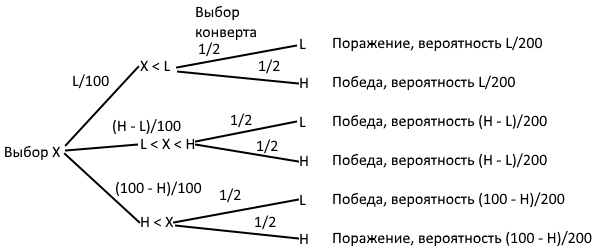
\includegraphics[width=\linewidth]{Envelopes.png}
\caption{Дерево вариантов}
\label{fig:Envelopes}
\end{figure}
Итак, посчитаем вероятность победы с использованием данной стратегии:\\
$Pr\{$победить$\} = \frac{L}{200} + \frac{H - L}{200} + \frac{H - L}{200} + \frac{100 - H}{200} = \frac{100 - H + H - L + L}{200} + \frac{H - L}{200} = \frac{1}{2} + \frac{H - L}{200}$,\\
то есть даже в худшем случае, когда противник выбрал два соседних числа, вероятность победить, используя данную стратегию составляет $50\frac{1}{2}\%$.
\subsubsection{Дискретная случайная величина}
Для вероятностного пространства $(S, Pr)$, $|S| < \infty$ функция $\xi: \; S \rightarrow \mathbb{R}$ называется дискретной случайной величиной (далее - ДСВ).\\
$Pr\{\xi = a\} = Pr(\{\omega \in S \; : \; \xi(\omega) = a\})$\\
$Pr\{\xi \leq a\} = Pr(\{\omega \in S \; : \; \xi(\omega) leq a\})$\\
Например для вероятностного пространства, иллюстрирующего три броска монетки, можно ввести дискретную случайную величину $\phi$, отражающую количество выпавших орлов. Тогда, например, $Pr\{\phi = 2\} = Pr(\{$РОО,ОРО,ООР$\}) = \frac{3}{8}$
\subsubsection{Математическое ожидание ДСВ}
Математическим ожиданием (матожиданием) ДСВ $\xi$ на вероятностном пространстве $(S, Pr)$ называют\\
$E \xi = \sum\limits_{\omega \in S}\xi(\omega) * Pr(\{\omega\})$\\
Альтернативная формула матожидания:\\
$E \xi = \sum\limits_{a \in Im(\xi)} \sum_{\omega \in S, \xi(\omega) = a} a * Pr(\{\omega\}) = \sum\limits_{a \in Im(\xi)} a * \sum_{\omega \in S, \xi(\omega) = a}Pr(\{\omega\}) = \sum\limits_{a \in Im(\xi)} a * Pr(\{\omega \in S \; : \; \xi(\omega) = a\}) = \sum\limits_{a \in Im(\xi)} a * Pr\{\xi = a\}$\\
Также можно заметить, что если изобразить числовую прямую как балку, и на каждой точке a из $Im(\xi)$ нарисовать столбик высоты $Pr\{\xi = a\}$, матожидание $\xi$ будет лежать на числовой прямой в той точке, на которой эту балку можно сбалансировать.\\
Вот рисунок для матожидания количества орлов, выпавших после броска трех монет:\\
\begin{figure}
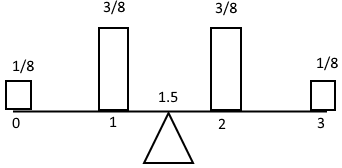
\includegraphics[width=\linewidth]{HeadsTails.png}
\caption{Матожидание количества орлов}
\label{fig:HeadsTails}
\end{figure}
\subsubsection{Арифметические действия с ДСВ и матожиданием}
\begin{itemize}
\item $\eta = \xi + c$ определим как $\eta(\omega) = \xi(\omega) + c$. $Pr\{\eta = a\} = Pr\{\xi + c = a\} = Pr\{\xi = a - c\}$. По второй формуле матожидания можно заметить, что $E \eta = c + E \xi$\\
\item $\eta = \xi * c$, $c \not= 0$ определим как $\eta(\omega) = \xi(\omega) * c$. $Pr\{\eta = a\} = Pr\{\xi * c = a\} = Pr\{\xi = \frac{a}{c}\}$. По второй формуле матожидания можно заметить, что $E \eta = c * E \xi$\\
\item $\eta = \xi^2$ определим как $\eta(\omega) = (\xi(\omega))^2$. $Pr\{\eta = a\} = Pr\{\xi^2 = a\}$. $E \eta = \sum\limits_{\omega \in S}\xi^2(\omega) * Pr(\{\omega\})$\\
\item $\eta = \xi + \psi$ определим как $(\xi + \psi)(\omega) = \xi(\omega) + \psi(\omega)$. $E (\\xi + \psi) = \sum\limits_{\omega \in S} (\xi(\omega) + \psi(\omega)) * Pr(\{\omega\}) = \sum\limits_{\omega \in S} \xi(\omega) * Pr(\{\omega\}) + \sum\limits_{\omega \in S} \psi(\omega) * Pr(\{\omega\}) = E \xi + E \psi$
\end{itemize}
\subsubsection{Дисперсия ДСВ}
Дисперсией ДСВ называют матожидание квадрата разности значения ДСВ и ее матожидания:\\
$D \xi = E (\xi - E \xi)^2$.\\
$E (\xi - E \xi)^2 = E (\xi^2 - 2 * E \xi * \xi + (E \xi)^2) = E \xi^2 - E (2 * E \xi * \xi)) + E (E \xi)^2 = E \xi^2 - 2 * E \xi * E \xi + (E \xi)^2 = E \xi^2 - (E \xi)^2$\\
Таким образом, $D \xi = E \xi^2 - (E \xi)^2$.